\documentclass[aspectratio=169]{beamer}
%
% Choose how your presentation looks.
%
% For more themes, color themes and font themes, see:
% http://deic.uab.es/~iblanes/beamer_gallery/index_by_theme.html
%
\mode<presentation>
{
  \usetheme{default}      % or try Darmstadt, Madrid, Warsaw, ...
  \usecolortheme{default} % or try albatross, beaver, crane, ...
  \usefonttheme{default}  % or try serif, structurebold, ...
  \setbeamertemplate{navigation symbols}{}
  \setbeamertemplate{caption}[numbered]
} 

% Set background to black and text to white
\setbeamercolor{background canvas}{bg=black}
\setbeamercolor{normal text}{fg=white}
\setbeamercolor{frametitle}{fg=white}
\setbeamercolor{title}{fg=white}

% You can continue to set other colors as needed:
\setbeamercolor{item}{fg=magenta} % Color of bullets
\setbeamercolor{subitem}{fg=yellow}
\setbeamercolor{subsubitem}{fg=cyan}
% ...
\setbeamertemplate{frametitle}[default][center]

\usepackage[english]{babel}
\usepackage[utf8]{inputenc}
\usepackage[T1]{fontenc}
\usepackage{graphicx}

% Set larger font for frame title
\setbeamerfont{frametitle}{size=\huge}

\usepackage{emoji}

\begin{document}

\begin{frame}
    \centering
    \Huge TikTok Successor Proposal \\

\includegraphics[width=0.3\textwidth]{imgs/app_icons/tiktok-icon2.png}
\end{frame}

\begin{frame}{Table of Contents}
\begin{columns}[T]
    \begin{column}[T]{0.5\textwidth}
        \begin{enumerate}
            \item Why replace TikTok?
            \item Weird groupchats 
            \item Beyond vertical video
            \item Power to the people
            \item Redesigned Algorithm
            \item Misc / How to help
        \end{enumerate}
    \end{column}
    \begin{column}{0.5\textwidth}
        
\includegraphics[height=0.8\textheight]{imgs/app_icons/tiktok-icon2.png}
    \end{column}
\end{columns}
\end{frame}

\begin{frame}{Why Replace TikTok?}
\begin{columns}[T]
    \begin{column}[T]{0.5\textwidth}
        \begin{itemize}
            \item Susceptible to 
            \begin{itemize}
                \item government control 
                \begin{itemize}
                    \item US Ban %%(bc \emoji{watermelon})
                    \item China 1hr/day limit
                    \item France \& Caledonia??
                \end{itemize}
                \item corporate greed
            \end{itemize}
            \item Need to make nobody in charge
            \begin{itemize}
                \item Solved in Part 4
            \end{itemize}
        \end{itemize}
    \end{column}
    \begin{column}{0.5\textwidth}
        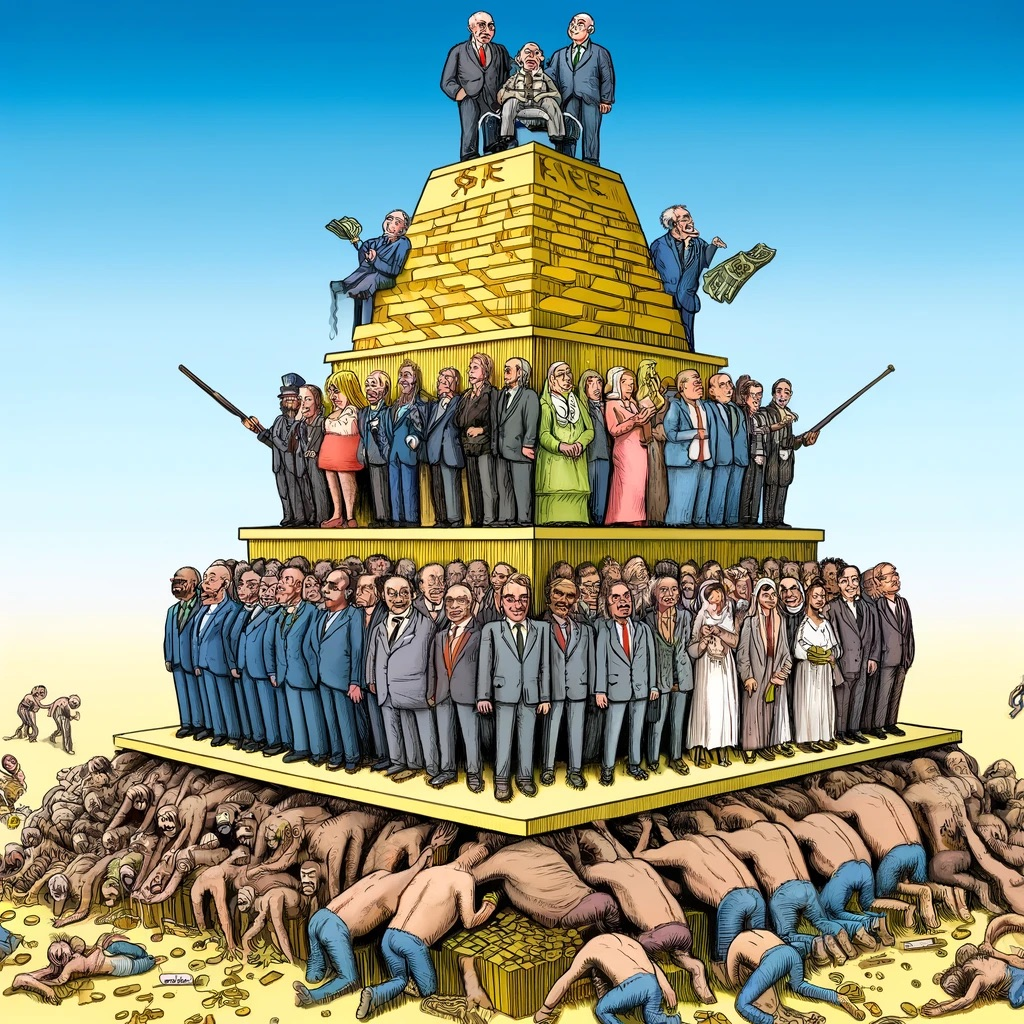
\includegraphics[height=0.8\textheight]{imgs/why_replace/power_pyramid.jpeg}
    \end{column}
\end{columns}
\end{frame}

\begin{frame}{A (Rough) History of Communication}
\vspace{-0.6in}
\begin{enumerate}
    \item Pre-internet info tech (ex. printing press, telegram) limited by bandwidth/access
        \begin{itemize}
            \item Increased info propagation $\rightarrow$ societal change (ex. free press \& Indian independence)
        \end{itemize}
    \item Facebook invented online friends (1-to-1 information propagation)
    \item Youtube/Instagram created influencers (1-to-all \textit{for some})
    \item Reddit developed shared-interest communities (group-to-1)
    \item Tiktok facilitated global consciousness (all-to-1)/(1-to-all \textit{for everybody})
    %%\begin{itemize}\item hence \emoji{watermelon} awareness\end{itemize}
    \item We need (all-to-all), (group-to-all), (1-to-group), (group-to-group)
    \begin{itemize}
        \item Solved in Parts 2 \& 5
    \end{itemize}
\end{enumerate}
\end{frame}

\begin{frame}{Misinformation}
\begin{columns}[T]
    \begin{column}[T]{0.5\textwidth}
        \begin{itemize}
            \item True of all social media
            \begin{itemize}
                \item Tiktok (debatably) worse
                \begin{itemize}
                    \item short video $\rightarrow$ difficult to cite
                    \item app difficult to navigate
                \end{itemize}
            \item AI makes this scarier
            \end{itemize}
        \item Need more media types
        \begin{itemize}
            \item Solved in Part 3
        \end{itemize}
    \end{itemize}
    \end{column}
    \begin{column}{0.5\textwidth}
        
\includegraphics[height=0.8\textheight]{imgs/why_replace/pope.png}
    \end{column}
\end{columns}
\end{frame}

\begin{frame}{Algorithms $\rightarrow$ Echo Chambers}
\begin{columns}[T]
    \begin{column}[T]{0.5\textwidth}
        \begin{itemize}
            \item True of all social media
            \begin{itemize}
                \item addiction = \$
            \end{itemize}
            \item Need to \textit{\textbf{optionally}} expose users to diverse viewpoints
            \begin{itemize}
                \item Solved in Part 5
            \end{itemize}
        \end{itemize}
    \end{column}
    \begin{column}{0.5\textwidth}
        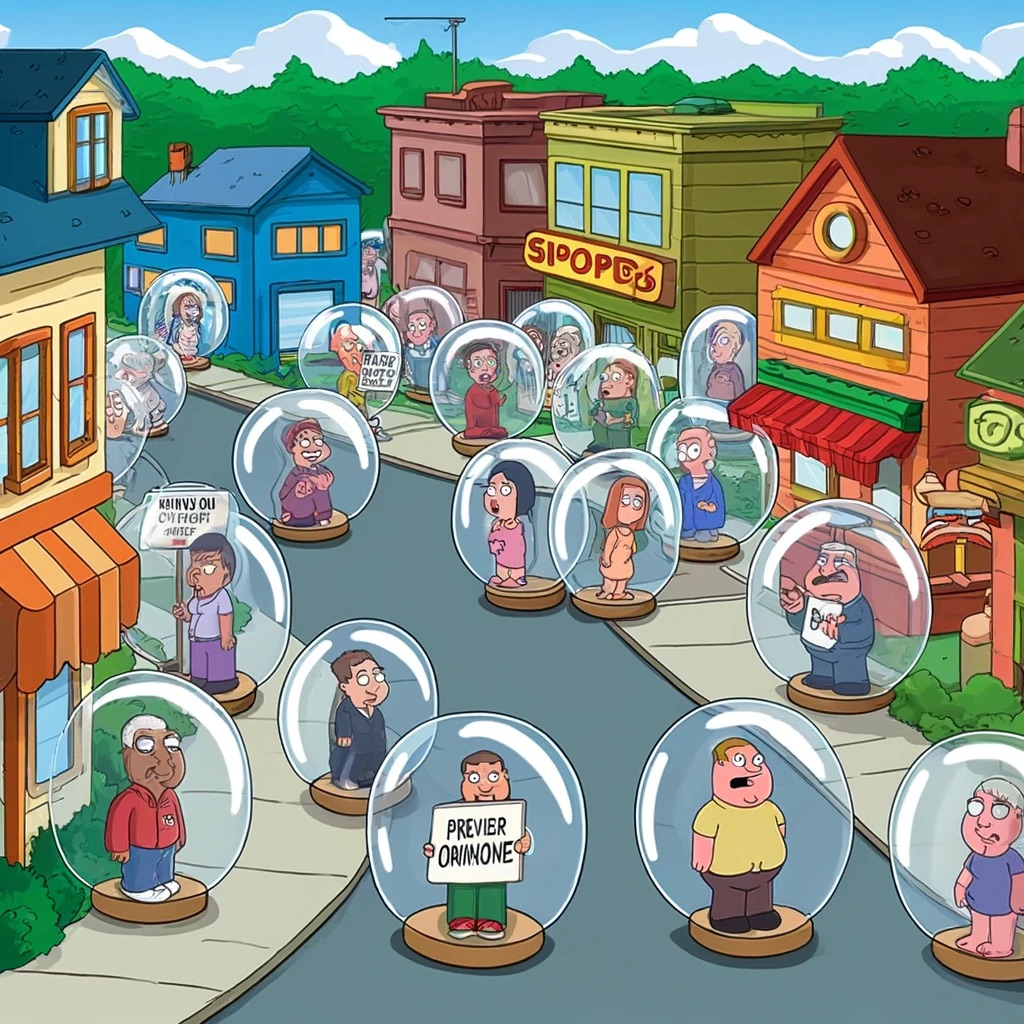
\includegraphics[height=0.8\textheight]{imgs/why_replace/bubble_town.jpeg}
    \end{column}
\end{columns}
\end{frame}

\begin{frame}{Why Replace TikTok?}
\begin{columns}[T]
    \begin{column}[T]{0.5\textwidth}
        \vspace{0.5in}
        \begin{itemize}
            \item Not the end of history
            \begin{itemize}
                \item Why not try to improve?
            \end{itemize}
        \end{itemize}
    \end{column}
    \begin{column}{0.5\textwidth}
        
\includegraphics[height=0.8\textheight]{imgs/why_replace/future_path.jpeg}
    \end{column}
\end{columns}
\end{frame}

\begin{frame}
    \centering
    \Huge TikTok Successor Proposal \\
    \Huge (Part 2: Weird Groupchats)
\end{frame}

\begin{frame}{Human Communication Has A Problem}
\begin{columns}[T]
    \begin{column}[T]{0.5\textwidth}
        \begin{itemize}
            \item Lots of us \& some louder than others
            \begin{itemize}
                \item Good ideas get over-shadowed
            \end{itemize}
            \item Can't coordinate without leadership
            \begin{itemize}
                \item Few points of failure
            \end{itemize}
            \item Time wasted listening \& filtering instead of deciding \& doing
        \end{itemize}
    \end{column}
    \begin{column}{0.5\textwidth}
        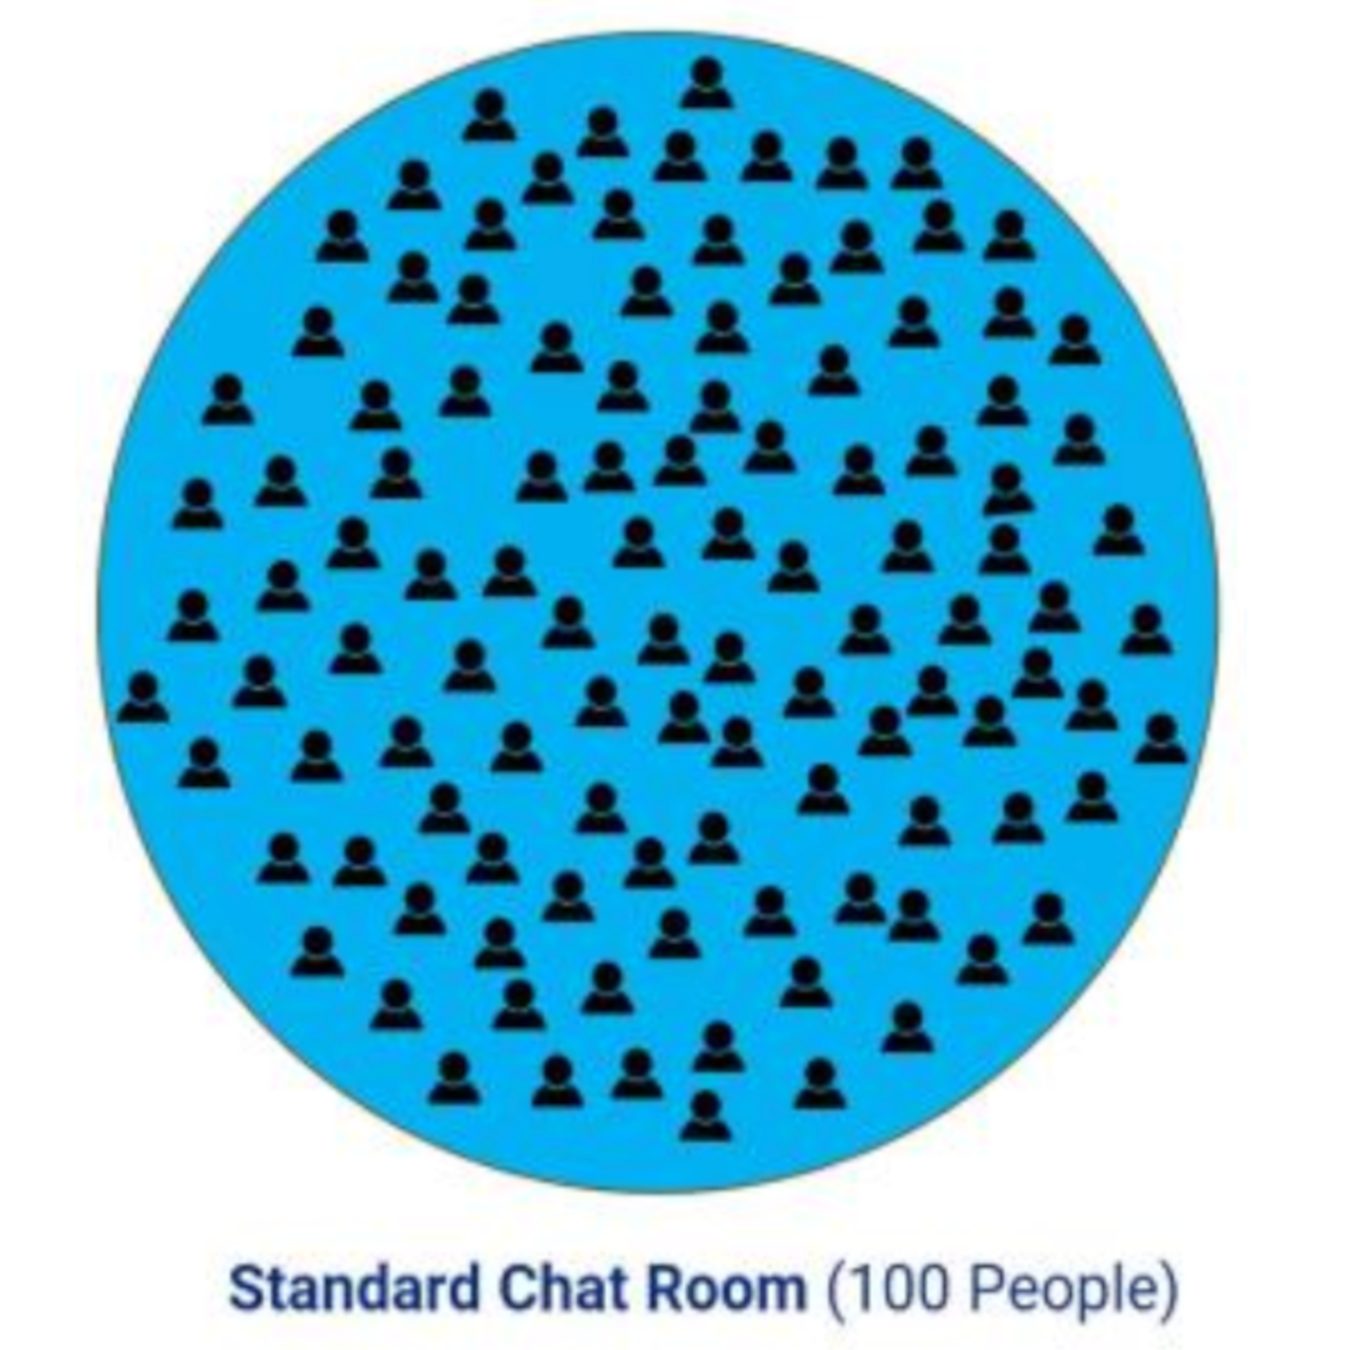
\includegraphics[height=0.8\textheight]{imgs/CSI_section/standard_chat_room.png}
    \end{column}
\end{columns}
\end{frame}

\begin{frame}{Conversational Swarm Intelligence (CSI)}
\begin{columns}[T]
    \begin{column}[T]{0.5\textwidth}
        \begin{itemize}
            \item Break into 20 groupchats of 5 people
            \item ChatGPT periodically summarizes
            \item Other groups receive those summaries
            \item Talk about each others' summaries
            \item After a few exchanges, info that sparks discussion will propagate
        \end{itemize}
    \end{column}
    \begin{column}{0.5\textwidth}
        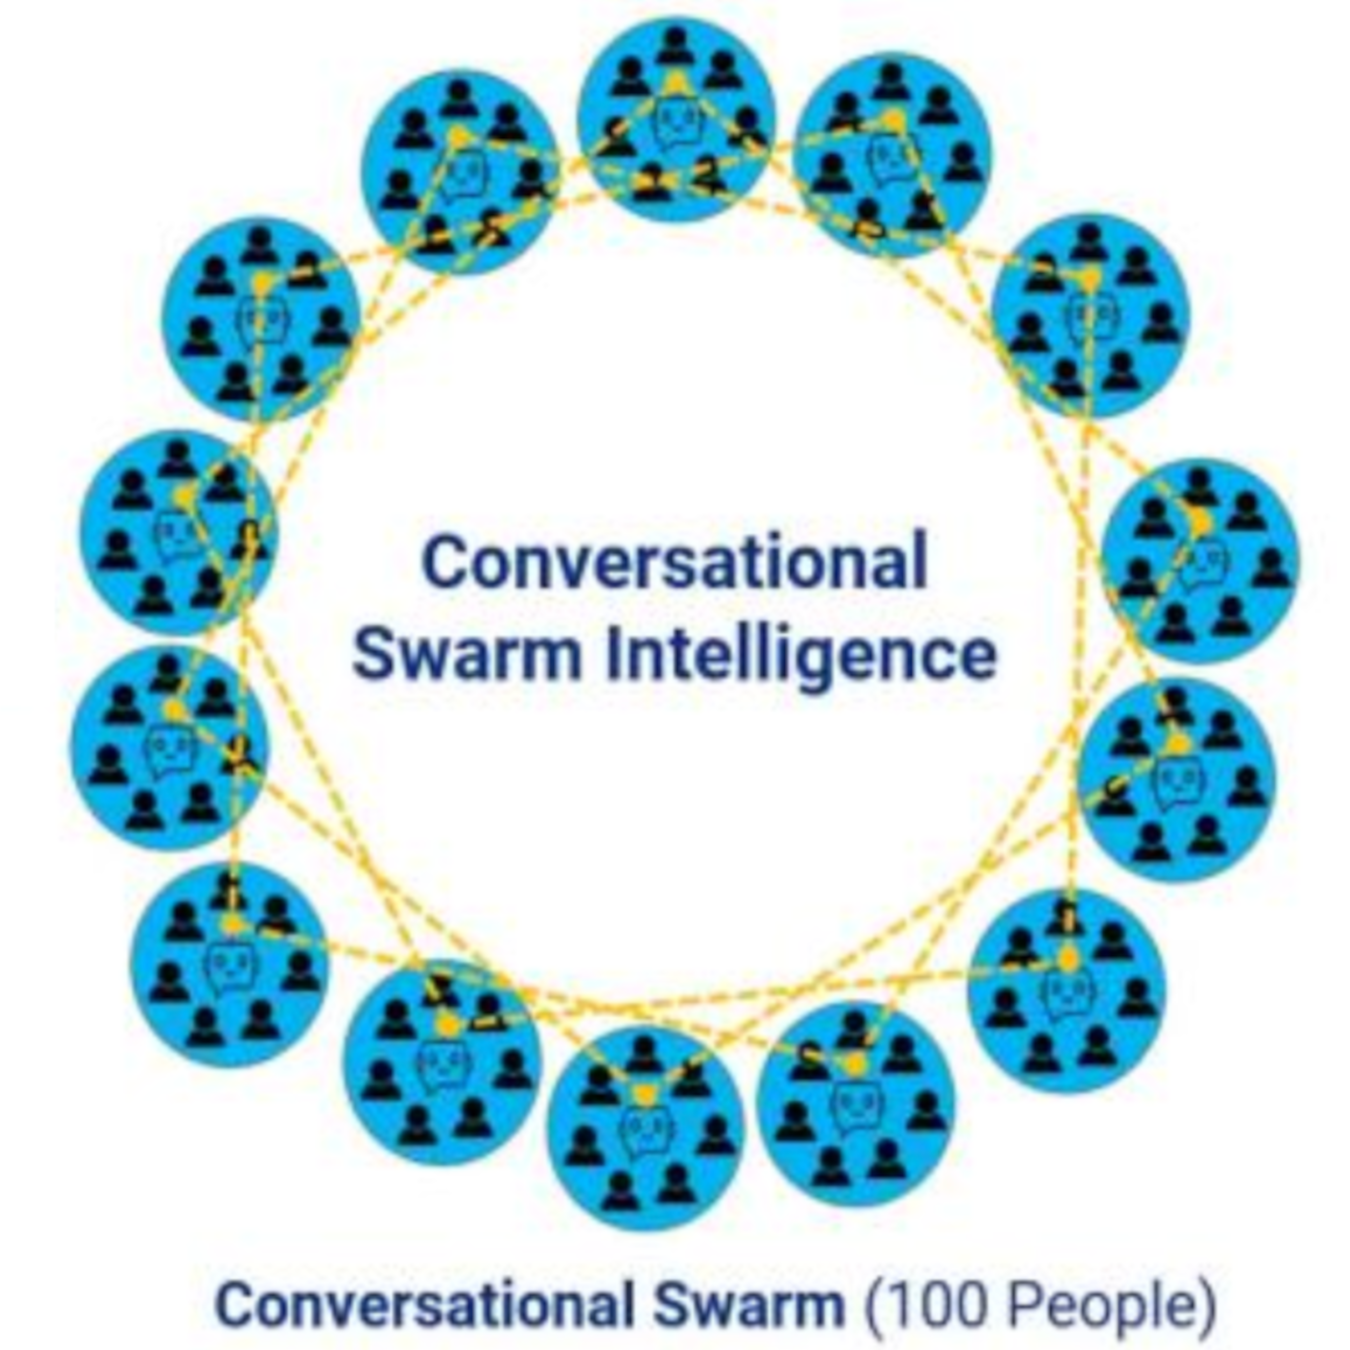
\includegraphics[height=0.8\textheight]{imgs/CSI_section/conversational_swarm.png}
    \end{column}
\end{columns}
\end{frame}

\begin{frame}{Credit}
\vspace{-0.5in}
\begin{center}
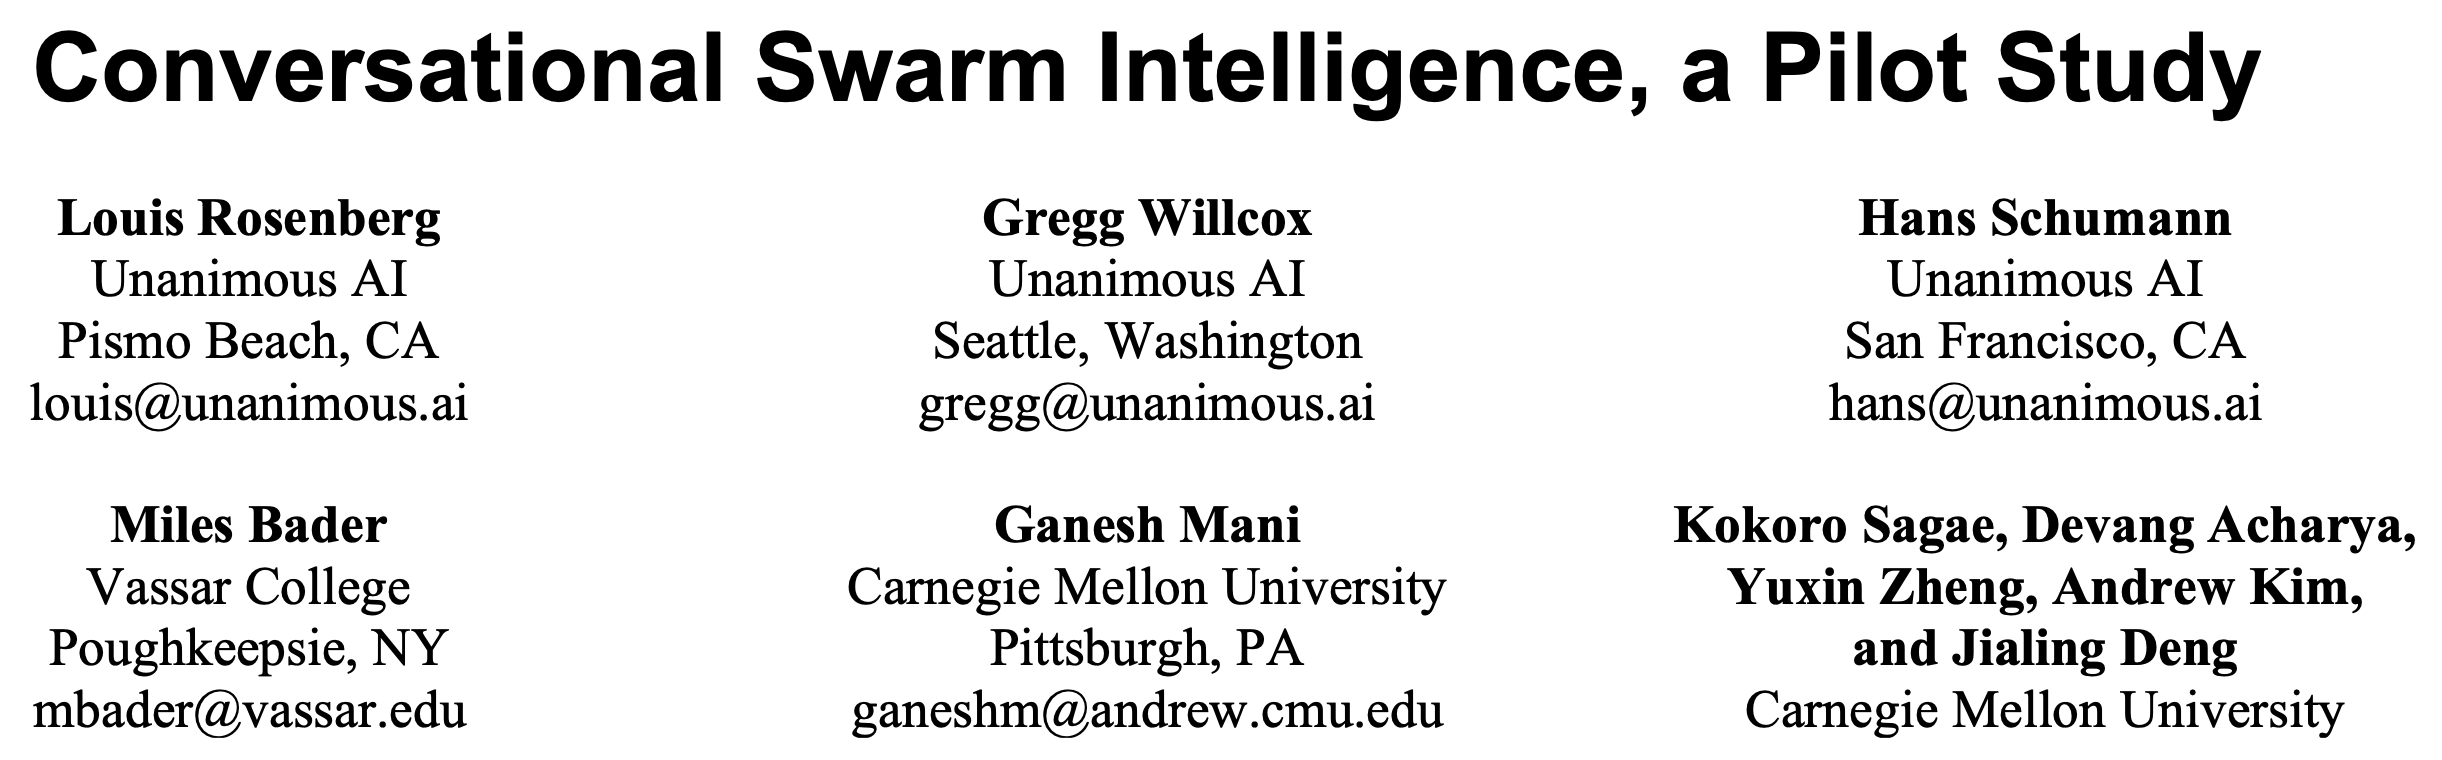
\includegraphics[width=\textwidth]{imgs/CSI_section/authors.png}
\end{center}
\end{frame}

\begin{frame}{Defining a "Summary"}
\begin{columns}[T]
    \begin{column}[T]{0.5\textwidth}
        \begin{itemize}
            \item Learns what you prefer over time
            \item You can directly edit / take over
        \end{itemize}
    \end{column}
    \begin{column}[T]{0.5\textwidth}
        \begin{itemize}
            \item Many settings to fiddle with
            \begin{itemize}
                \item frequency
                \item length
                \item group size
                \item what groups will you join
            \end{itemize}
            \item Customize the summary to your needs
            \begin{itemize}
                \item meeting minutes (historian)
                \item key takeaways / action items (intern)
                \item criticisms (devil's advocate)
                \item personalize to group that's receiving
            \end{itemize}
        \end{itemize}
    \end{column}
\end{columns}
\end{frame}

\begin{frame}{Hierarchical CSI}
\begin{columns}[T]
    \begin{column}[T]{0.5\textwidth}
        \begin{itemize}
            \item Scales up levels
            \item Groups of ANY size
            \item mix-n-match
        \end{itemize}
    \end{column}
    \begin{column}{0.5\textwidth}
        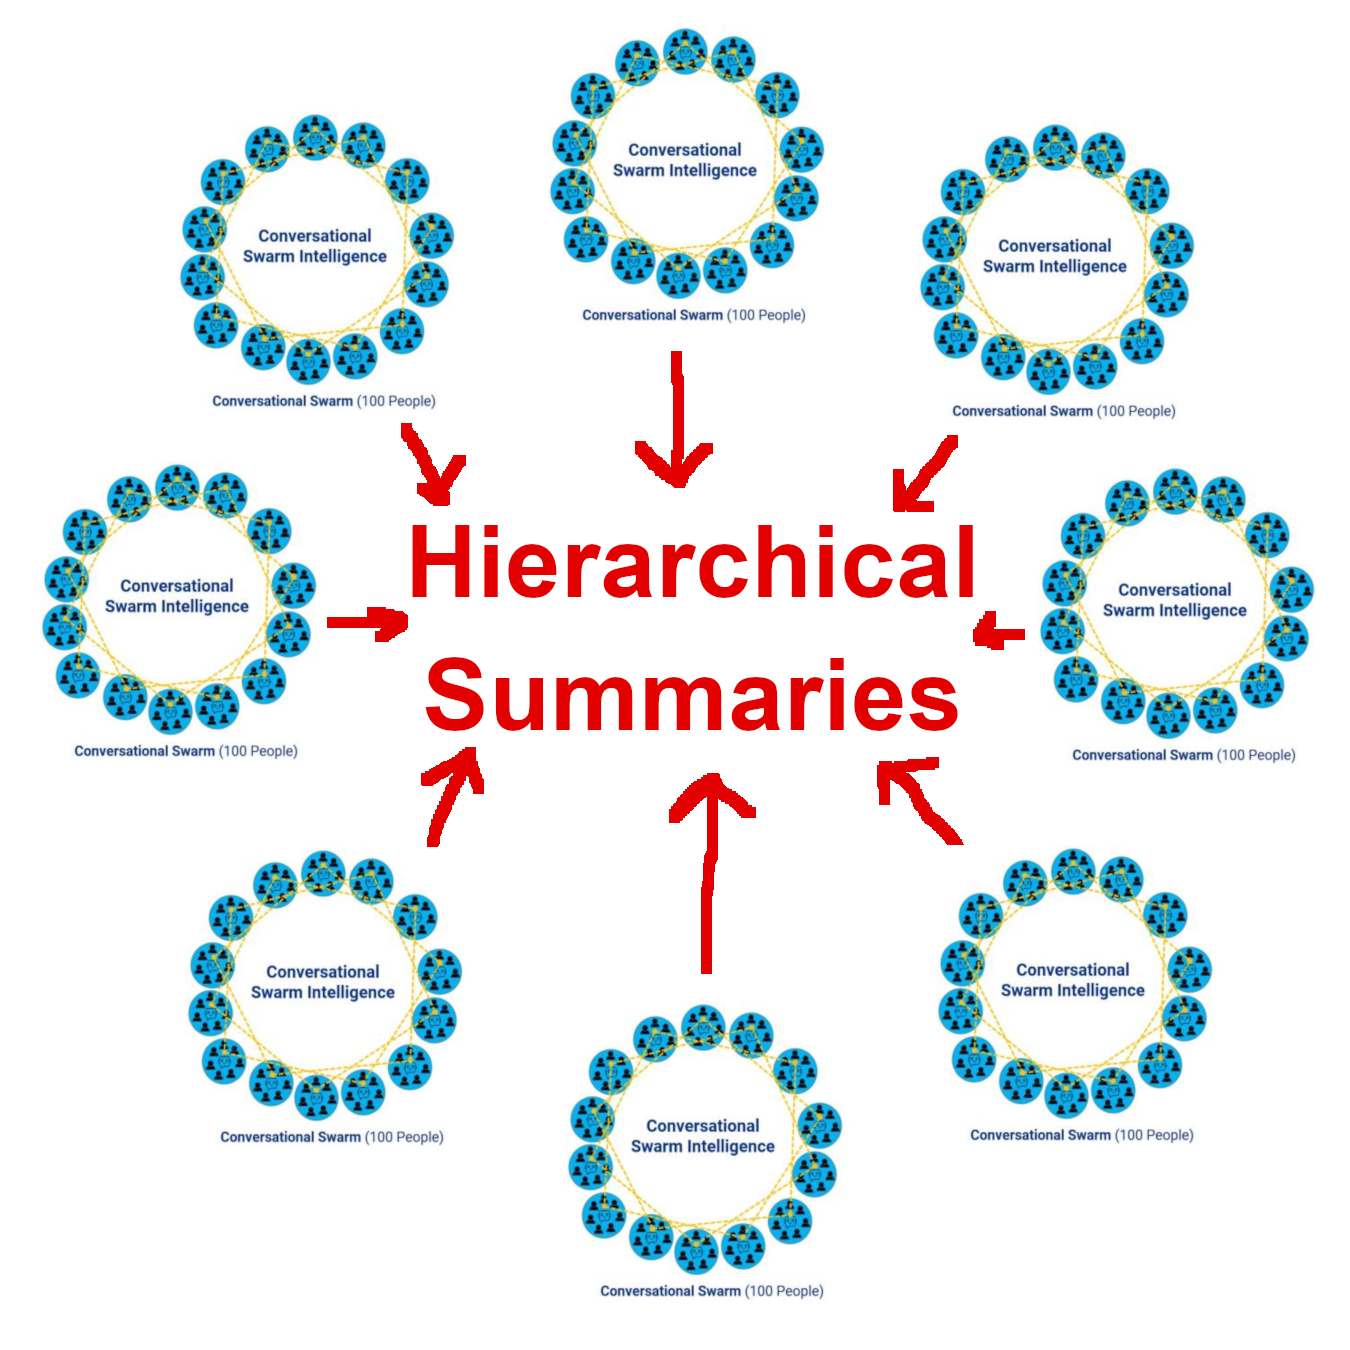
\includegraphics[height=0.8\textheight]{imgs/CSI_section/hierarchical_summaries.png}
    \end{column}
\end{columns}
\end{frame}

\begin{frame}{Interaction w/ World}
\begin{columns}[T]
    \begin{column}[T]{0.5\textwidth}
        \begin{itemize}
            \item talk with an \textit{<insert group name here>}GPT instead of an actual person in that group
            \begin{itemize}
                \item be exposed to groups you otherwise have no familiarity with / access to
            \end{itemize}
            \item making a public GPT for your group is COMPLETELY OPTIONAL
        \end{itemize}
    \end{column}
    \begin{column}{0.5\textwidth}
        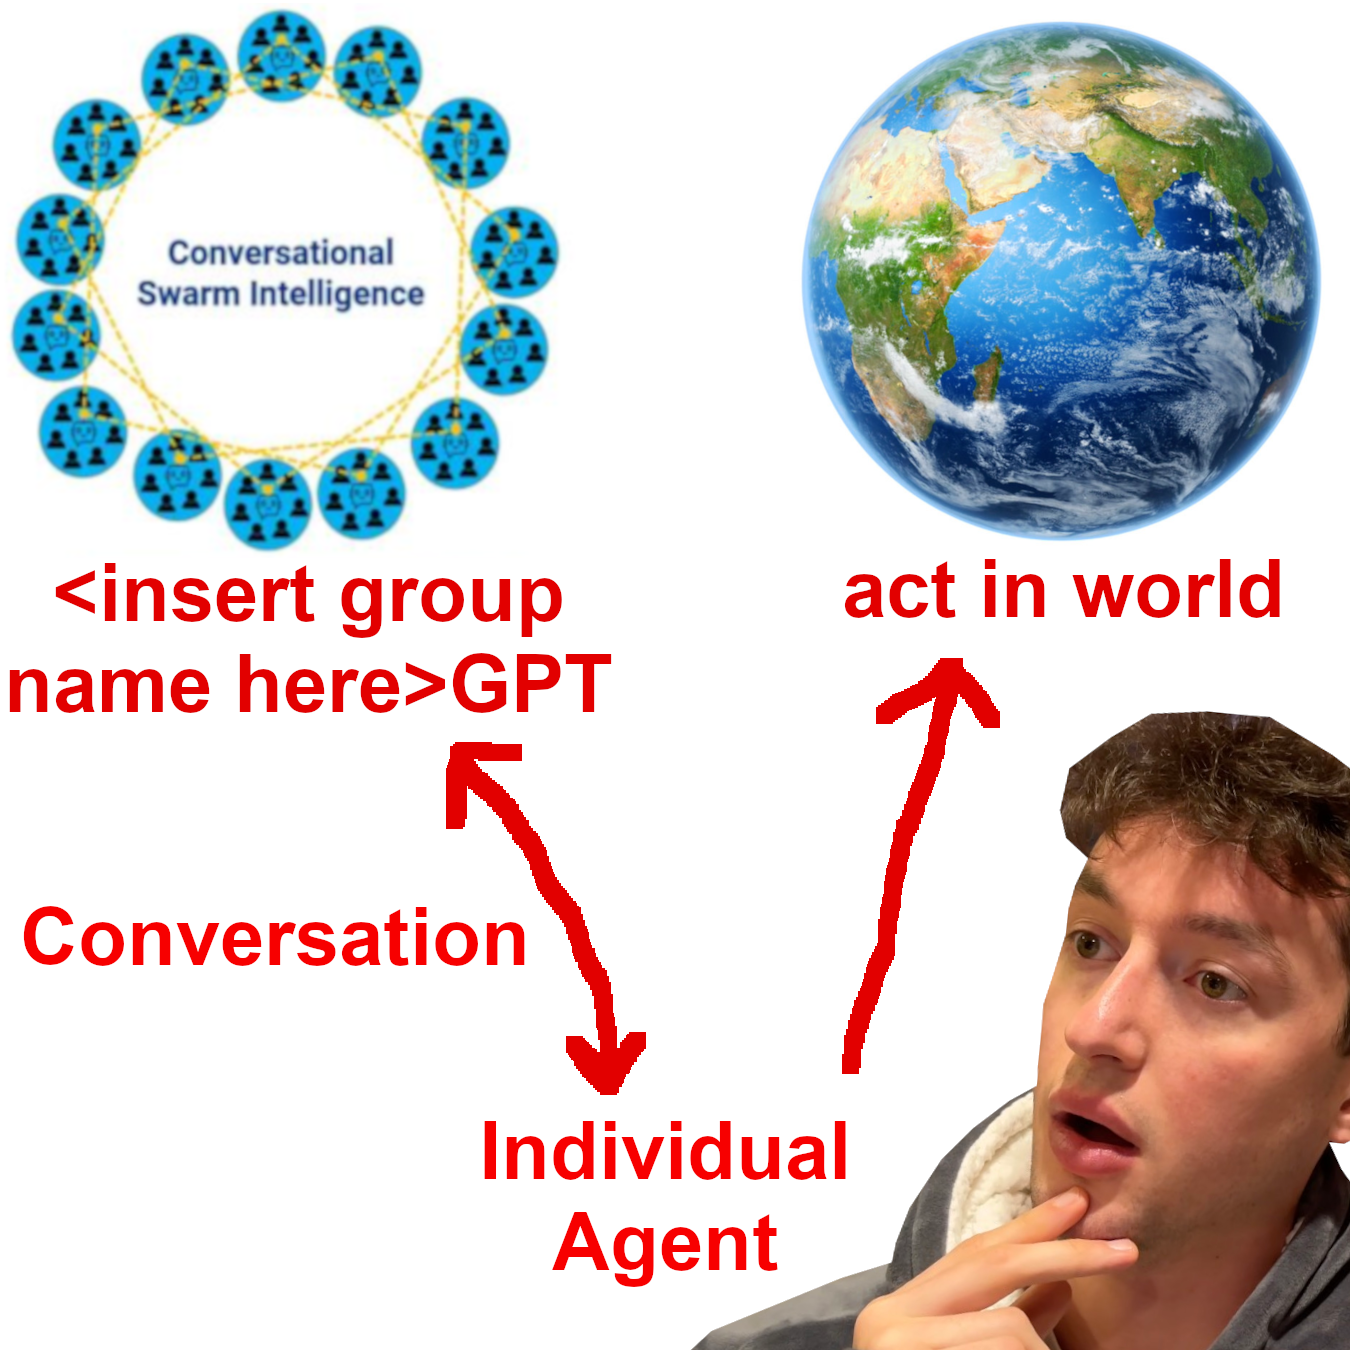
\includegraphics[height=0.8\textheight]{imgs/CSI_section/agency.png}
    \end{column}
\end{columns}
\end{frame}

\begin{frame}{Target Audiences / Use Cases}
\begin{columns}[T]
    \begin{column}[T]{0.5\textwidth}
        \begin{itemize}
            \item Online shared interest communities
            \item Local community organization
            \item Replace middle-management
            \item Grassroots movements won't need leaders or centralized decision making
            \item Literally any large group of people
        \end{itemize}
    \end{column}
    \begin{column}{0.5\textwidth}
        
\includegraphics[height=0.8\textheight]{imgs/CSI_section/competition.png}
    \end{column}
\end{columns}
\end{frame}

\begin{frame}
    \centering
    \Huge TikTok Successor Proposal \\
    \Huge (Part 3: Beyond Short Vertical Videos)
\end{frame}

\begin{frame}{What stays the same}
\begin{columns}[T]
    \begin{column}[T]{0.5\textwidth}
        \begin{itemize}
            \item Short-form vertical video
            \item Algorithm-driven
            \begin{itemize}
                \item More on this in Part 5
            \end{itemize}
        \end{itemize}
    \end{column}
    \begin{column}{0.5\textwidth}
        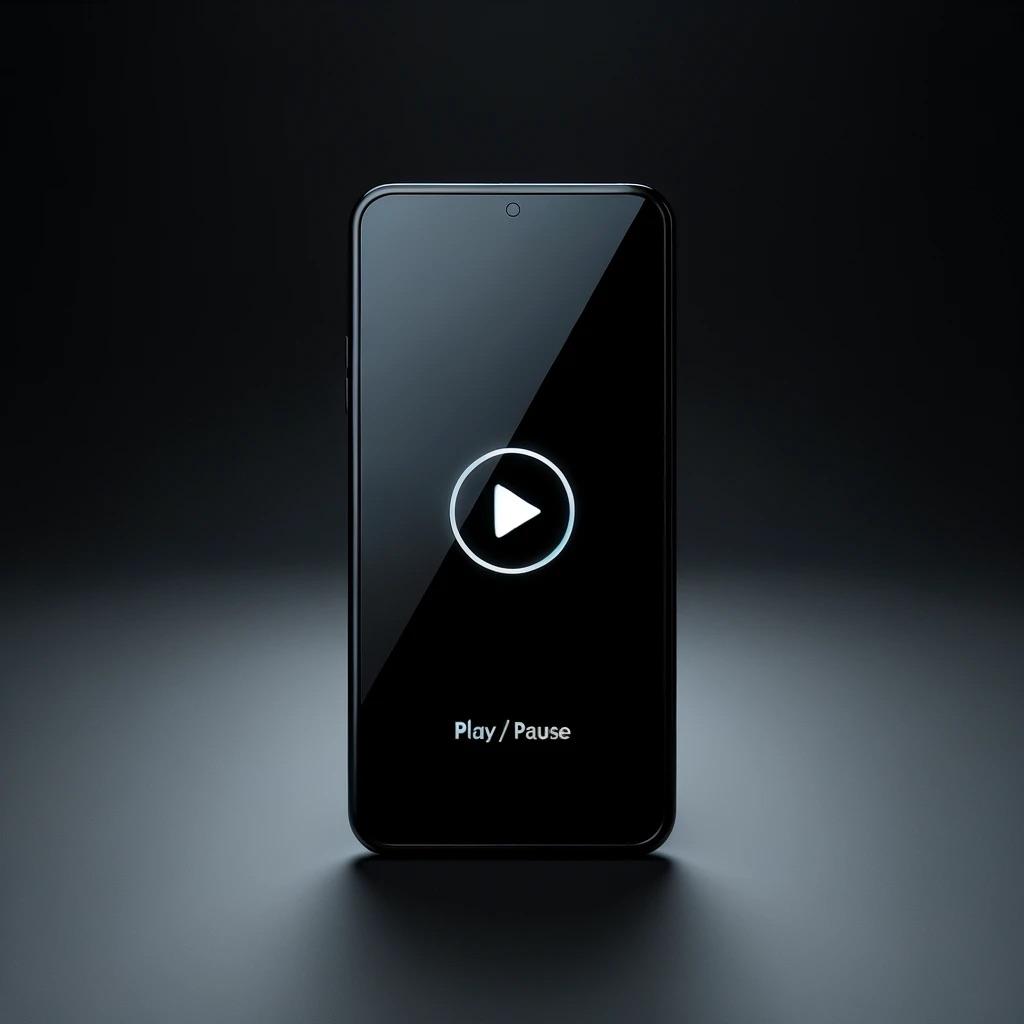
\includegraphics[height=0.8\textheight]{imgs/media/vertical_vid.jpeg}
    \end{column}
\end{columns}
\end{frame}

\begin{frame}{Horizontal Video}
\begin{columns}[T]
    \begin{column}[T]{0.5\textwidth}
        \begin{itemize}
            \item Just rotate your phone
                \item Longer-form content
                \item Introduces whole different culture
                \begin{itemize}
                    \item higher detail/quality/rigor/length
                \end{itemize}
        \end{itemize}
    \end{column}
    \begin{column}{0.5\textwidth}
        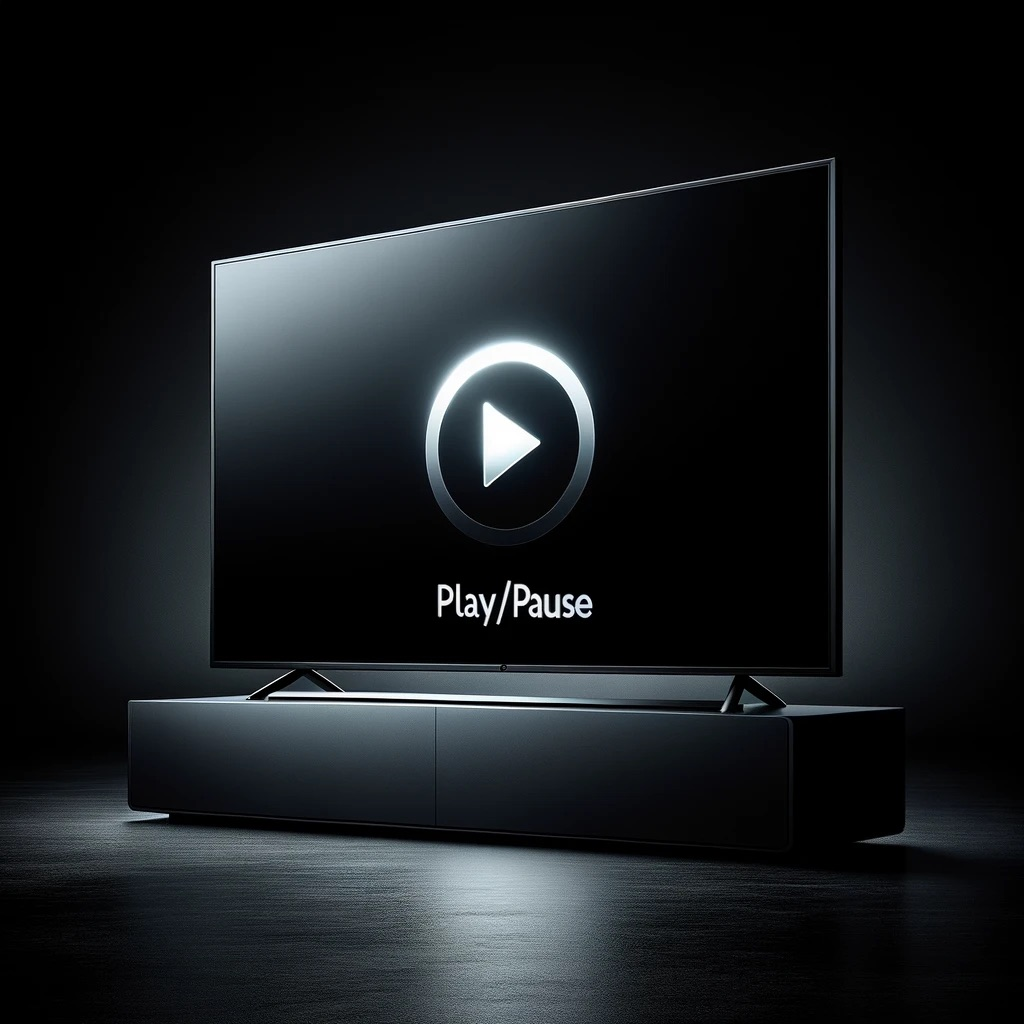
\includegraphics[height=0.8\textheight]{imgs/media/horizontal_vid.jpeg}
    \end{column}
\end{columns}
\end{frame}

\begin{frame}{Written Articles}
\begin{columns}[T]
    \begin{column}[T]{0.5\textwidth}
        \begin{itemize}
            \item Include actual links to sources
            \item Invites "legit" (traditional) journalism
            \item Literally just in your FYP feed
            \item Comment/stitch them to videos
            \item TLDR for me, but Nerds will love
            \item Also tweet-length stuff
        \end{itemize}
    \end{column}
    \begin{column}{0.5\textwidth}
        
\includegraphics[height=0.8\textheight]{imgs/media/quil.png}
    \end{column}
\end{columns}
\end{frame}

\begin{frame}{Conversational Swarm Integration}
\begin{columns}[T]
    \begin{column}[T]{0.5\textwidth}
        \begin{itemize}
            %\item Watch Part 2 for this to make sense
            \item Alongside "FYP", "Following", and "STEM" each swarm you're part of will have its own vertical scroll feed
        \end{itemize}
    \end{column}
    \begin{column}{0.5\textwidth}
        \begin{itemize}
            \item In livestreams, the streamer can talk with a swarm summary of the viewers
            \item In groupchats, a ChatGPT can (optionally) be on standby to send videos \& articles relevant to your conversation
            \begin{itemize}
                \item inspiration
                \item fact-checking
                \item counter-arguments
            \end{itemize}
        \end{itemize}
    \end{column}
\end{columns}
\end{frame}

\begin{frame}
    \centering
    \Huge TikTok Successor Proposal \\
    \Huge (Part 4: Power to the people)
\end{frame}

\begin{frame}{Modularity/Choice}
\begin{columns}[T]
    \begin{column}[T]{0.5\textwidth}
        \begin{itemize}
            \item EVERYTHING is optional; \\turn anything off
            \begin{itemize}
                \item Data privacy
                \item May reduce experience
            \end{itemize}
            \item Swap-out any feature for one someone else made
            \begin{itemize}
                \item Algorithms
            \end{itemize}
        \end{itemize}
    \end{column}
    \begin{column}{0.5\textwidth}
        
\includegraphics[height=0.8\textheight]{imgs/power_to_people/legos.png}
    \end{column}
\end{columns}
\end{frame}

\begin{frame}{Open-Source}
\vspace{-0.3in}
\begin{columns}[T]
    \begin{column}[T]{0.5\textwidth}
        \begin{itemize}
            \item Definition: all code is released to the internet, free for anyone to use
            \begin{itemize}
                \item Nerds don't need profit incentive to make cool things
            \end{itemize}
            \item Open-source as many parts as possible, maybe even whole thing
            \item Companies, organizations, nerds, etc can build their own versions
        \end{itemize}
    \end{column}
    \begin{column}{0.5\textwidth}
        
\includegraphics[width=\textwidth]{imgs/power_to_people/open-source.png}
    \end{column}
\end{columns}
\end{frame}

\begin{frame}{Encryption}
\vspace{-0.7in}
\begin{itemize}
    \item Encryption for privacy wherever possible
    \begin{itemize}
        \item Likely incompatible with some features, thus restricting quality of experience
        \begin{itemize}
            \item Some not enabled by default
        \end{itemize}
    \end{itemize}
    \item Encryption + Conversational Swarm $\rightarrow$ competes with Telegram \emoji{brain}\emoji{gear}
    \begin{itemize}
        \item Run your own local ChatGPT for Conversational Swarm and use it fully encrypted instead of our default model
    \end{itemize}
\end{itemize}
\end{frame}

\begin{frame}{Decentralization}
\begin{columns}[T]
    \begin{column}[T]{0.5\textwidth}
        \begin{itemize}
            \item Crypto\$ is cringe but hear me out
            \begin{itemize}
                \item No investment currency here
            \end{itemize}
            \item Underlying technology (blockchain) means NO ONE can control your info
            \item The FYP algorithm likely requires an organization/company/nerd to run
            \begin{itemize}
                \item Federated instead of flat
            \end{itemize}
        \end{itemize}
    \end{column}
    \begin{column}{0.5\textwidth}
        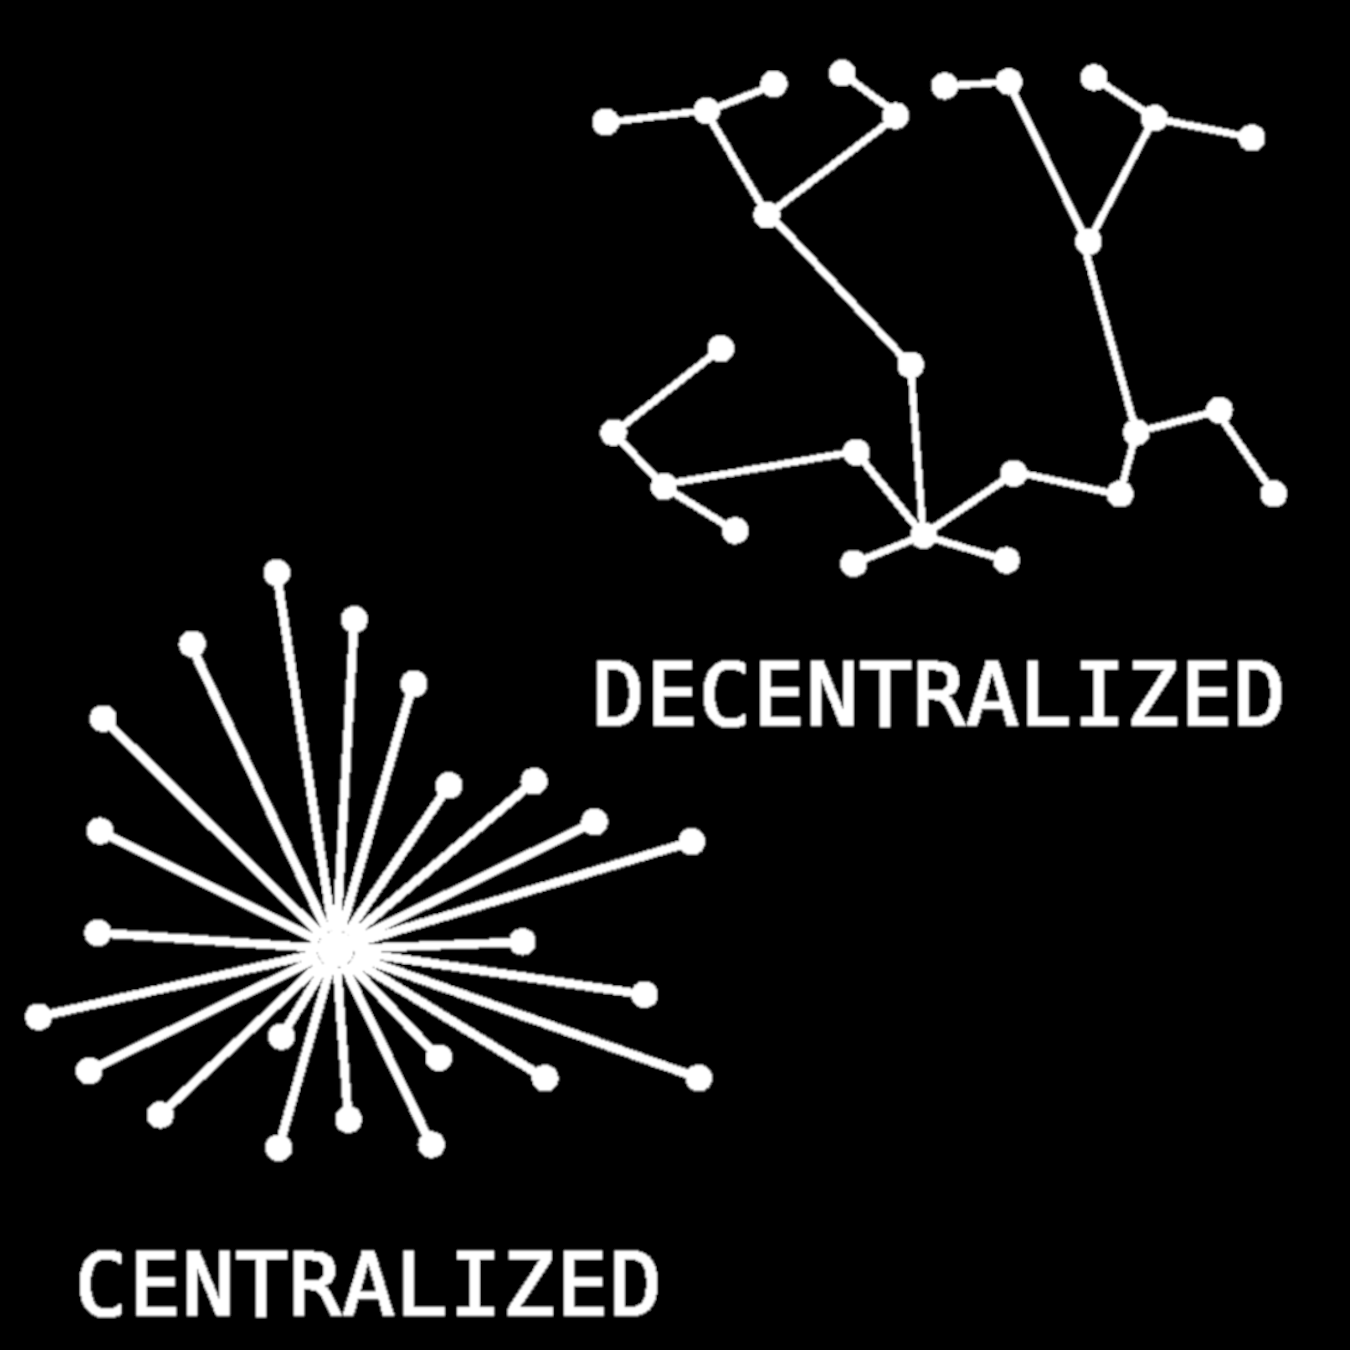
\includegraphics[height=0.8\textheight]{imgs/power_to_people/decentralized.png}
    \end{column}
\end{columns}
\end{frame}

\begin{frame}
    \centering
    \Huge TikTok Successor Proposal \\
    \Huge (Part 5: Redesigned Algorithm)
\end{frame}

\begin{frame}{Thesis}
\vspace{-0.8in}
\begin{itemize}
    \item Algorithms could be good (less bad) if there were no (less) profit incentive
    \item ***My expertise is in AI language models, not recommendation
 \end{itemize}
\end{frame}

\begin{frame}{Current Algorithm Dynamic}
\vspace{-0.6in}
\begin{enumerate}
    \item Companies want \$
    \item Advertising $\rightarrow$ \$
    \item Addicting you $\rightarrow$ more time for ads
    \item Our brains respond to sycophantic praise \& negative emotions (anger, fear, etc.)
    \item Algorithms usually trained to isolate you into a bubble and make you hate/fear people/ideas outside the bubble
\end{enumerate}
\end{frame}

\begin{frame}{TikTok's Algorithm}
\vspace{-0.6in}
TikTok still fundamentally works this way BUT
\begin{enumerate}
    \item Short-form video $\rightarrow$ more videos seen per hour
    \item More data $\rightarrow$ better algorithm
    \begin{itemize}
        \item Youtube only shows you what you already like
        \item TikTok introduces you to what you didn't know you would like
    \end{itemize}
    \item When a topic reaches critical mass it gets shown to people who have not previously displayed interest
    %%\begin{itemize}\item hence \emoji{watermelon}\end{itemize}
\end{enumerate}
\end{frame}

\begin{frame}{Swap out algorithms}
\vspace{-0.6in}
\begin{itemize}
    \item Simple ones run on gaming PCs
    \item Big AI ones need companies with supercomputers
    \begin{itemize}
        \item Incentivize providers with the right to serve ads
    \end{itemize}
    \item Also swap-out GPT models in conversational swarm
    \begin{itemize}
        \item Watch Part 2 to understand this point
    \end{itemize}
\end{itemize}
\end{frame}

\begin{frame}{Our Algorithm}
\vspace{-0.7in}
\begin{itemize}
    \item Default is similar to Tiktok's. These are \textbf{potential} \textit{options}:
    \begin{itemize}
        \item Show content it predicts you will \textit{not} like
        \item Occasionally show random content
        \item Only view local content
        \item Have it constantly try to change your mind
        \item Optimize for growth of your group
    \end{itemize}
    \item This is very TBD, idk exactly what's possible
\end{itemize}
\end{frame}

\begin{frame}
    \centering
    \Huge TikTok Successor Proposal \\
    \Huge (Part 6: Misc / How to Help)
\end{frame}

\begin{frame}{Potential Branding}
\vspace{-0.5in}
\begin{columns}[T]
    \begin{column}[T]{0.5\textwidth}
    Inspiration sources for names
        \begin{itemize}
            \item Intelligent swarm behavior in animals
            \item Bee hives
            \item Spider webs
            \item Chorus, harmonics
            \item Communication
            \item Cooperation
        \end{itemize}
    \end{column}
    \begin{column}{0.5\textwidth}
        \begin{tabular}{cccc}
            
\includegraphics[width=0.2\textwidth]{imgs/app_icons/7.png} & 
\includegraphics[width=0.2\textwidth]{imgs/app_icons/8.png} & 
\includegraphics[width=0.2\textwidth]{imgs/app_icons/1.png} & 
\includegraphics[width=0.2\textwidth]{imgs/app_icons/2.png}\\ 
            
\includegraphics[width=0.2\textwidth]{imgs/app_icons/3.png} & 
\includegraphics[width=0.2\textwidth]{imgs/app_icons/4.png} & 
\includegraphics[width=0.2\textwidth]{imgs/app_icons/5.png} & 
\includegraphics[width=0.2\textwidth]{imgs/app_icons/6.png}\\ 
        \end{tabular}
        Example Names
        \begin{itemize}
            \item World Web
            \item Tea Hive
            \item Harmonhive
        \end{itemize}
    \end{column}
\end{columns}
\end{frame}

\begin{frame}{Why Did I Post This?}
\vspace{-0.9in}
\begin{itemize}
    \item Open-sourcing everything is kinda my brand
    \begin{itemize}
        \item Please critique, suggest, etc
    \end{itemize}
    \item I don't have access to VC money
    \begin{itemize}
        \item Ideally this project would be completely community funded
    \end{itemize}
    \item I'm holding back heavy on the biggest parts of the idea
    \begin{itemize}
        \item If you try to beat me to it you're only helping me
    \end{itemize}
\end{itemize}
\end{frame}

\begin{frame}{Minimum Viable Products}
\vspace{-0.9in}
\begin{itemize}
    \item Discord bot
    \item Twitch stream
    \item Discord/Telegram/Slack competitor (ignore the TikTok part)
\end{itemize}
\end{frame}

\begin{frame}{How Can You Learn More / Help?}
\vspace{-0.9in}
\begin{itemize}
    \item Link in description to a google form
    \begin{itemize}
        \item Be put on email list for IF/when app comes out
        \item Contribute labor/code
        \item Contribute funding
        \item Contribute compute
    \end{itemize}
    \item Join the discord (link in description)
\end{itemize}
\end{frame}

\end{document}
